\subsection{Точки Лагранжа}

\term{Точки Лагранжа}~--- точки во вращающейся системе из двух массивных тел,
\begin{wrapfigure}[14]{l}{0.48\tw}
	\centering
	\vspace{-.5pc}
	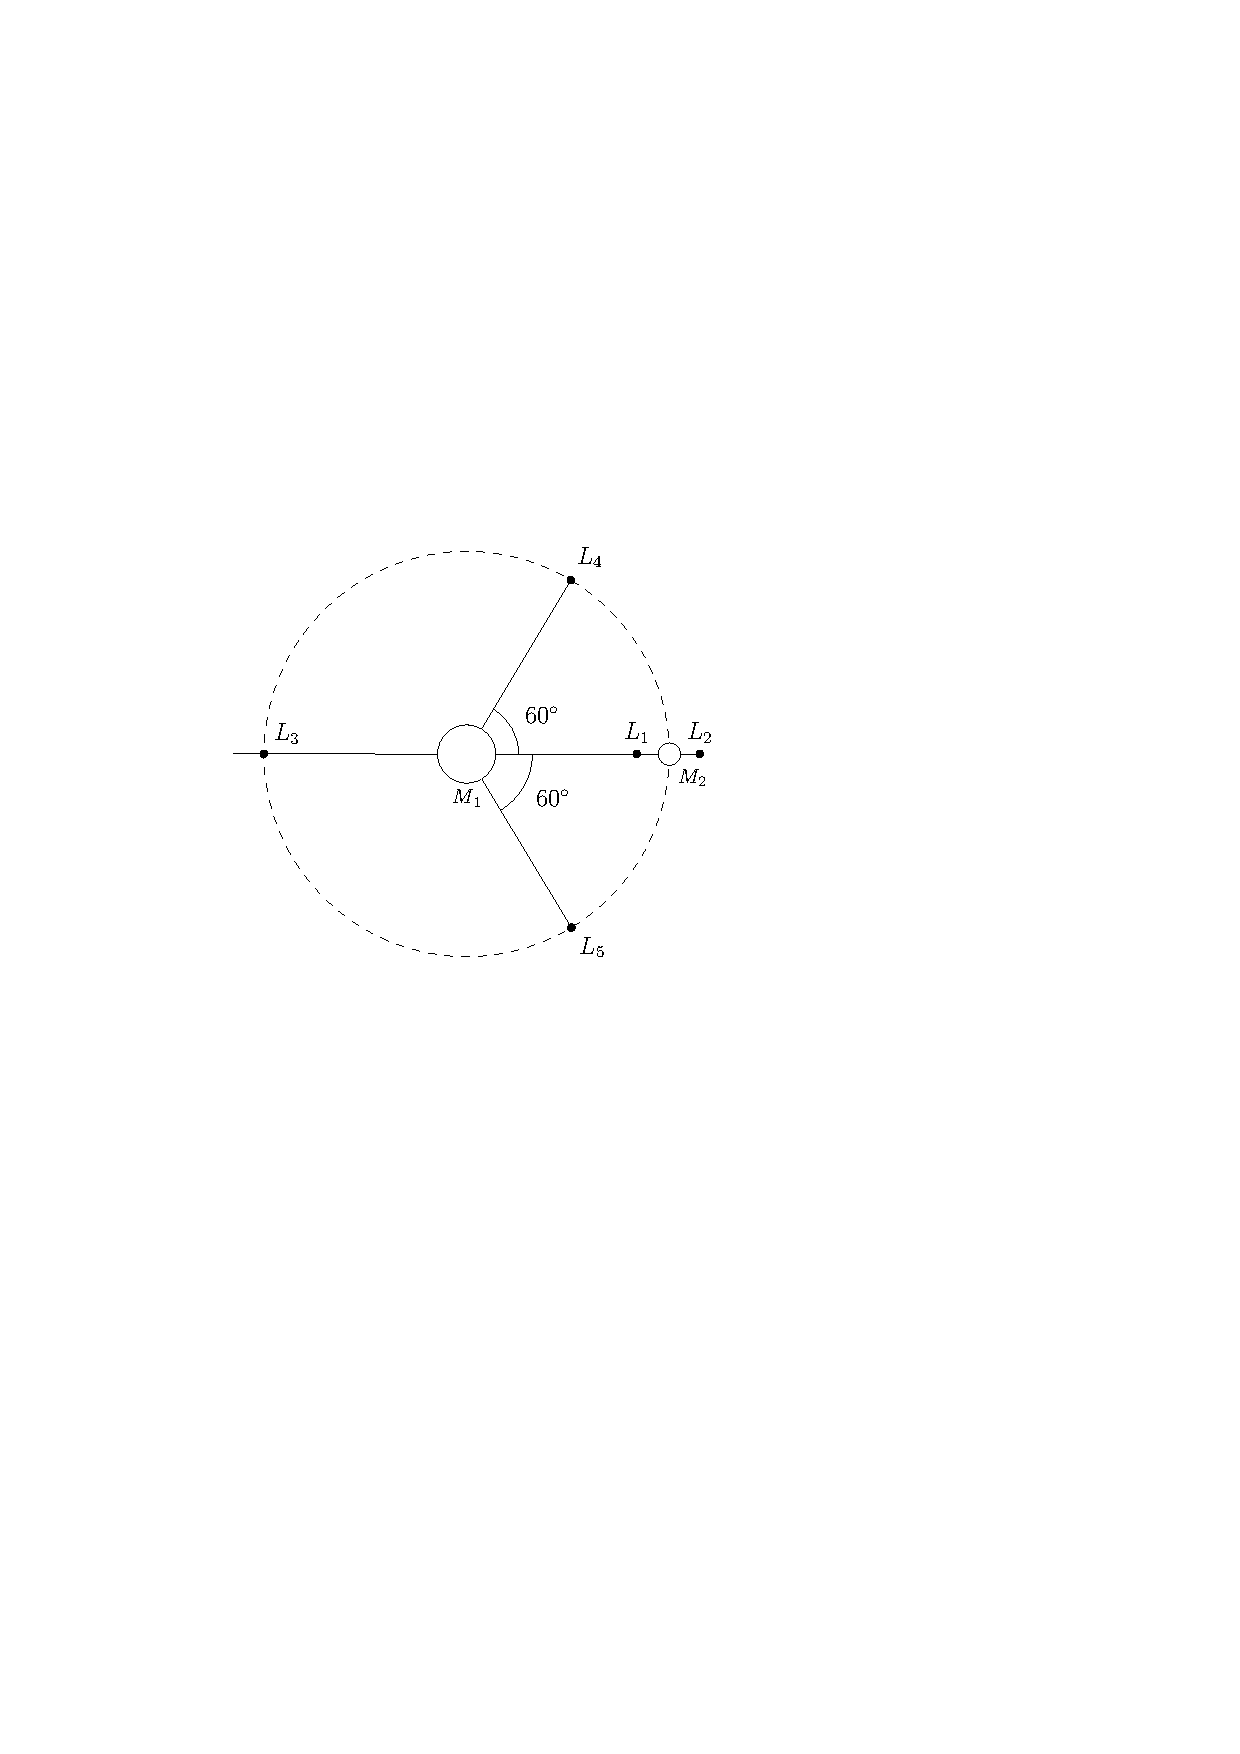
\includegraphics[width = .48\tw]{lagr-points}
	\captionof{figure}{Точки Лагранжа}
	\label{pic:larg-points}	
\end{wrapfigure}
в которых третье тело с пренебрежимо 
малой массой, не испытывающее воздействие никаких 
других сил, кроме гравитационных со стороны двух 
первых тел, может оставаться неподвижным относительно 
этих тел. В этих точках гравитационные силы, 
действующие на малое тело, уравновешиваются силами инерции.

Точки $L_1$, $L_2$ и $L_3$ лежат на одной прямой, 
соединяющей два массивных тела. Точки $L_4$ и $L_5$ 
образуют равносторнние треугольники с массивными 
телами.

Для расстояний до точек $L_1$, $L_2$ и $L_3$ от 
центра масс системы справедливы следующие выражения:
\begin{equation}r_1=R\left(1-\sqrt[3]{\frac{\alpha}
{3}}\right), \quad r_2=R\left(1+\sqrt[3]{\frac{\alpha}
{3}}\right), \quad r_3=R\left(1+\frac{5}{12}\alpha\right),
\end{equation}
где $\alpha=M_2 / (M_1 + M_2)$, $R$~--- расстояние между 
телами, $M_1$ --- масса более массивного тела, $M_2$
 --- масса второго тела.

Если $M_2 \ll M_1$, то точки $L_1$ и $L_2$ находятся 
примерно на одинаковом расстоянии от тела $M_2$, равном
\begin{equation}
r\approx R\sqrt[3]{\frac{M_2}{3M_1}}.
\end{equation}

Расстояния от центра масс системы до точек $L_4$ и $L_5$ в координатной системе с центром координат в центре масс системы рассчитываются по  формулам
\begin{equation}
	 r_4 = \left ( \frac{R}{2} \cdot \frac{M_1-M_2}{M_1+M_2} ,   \frac{\sqrt{3}R}{2} \right ), \quad r_5 = \left ( \frac{R}{2} \cdot \frac{M_1-M_2}{M_1+M_2} ,   -\frac{\sqrt{3}R}{2} \right ). 
\end{equation}